\chapter{Satellite capturing process}
\qquad \underline{By} : Julien \\
\label{sec:5}
\section{Choice of the process}

\qquad In order to capture and de-orbit a satellite in GEO, we considered the following usable tools :
\begin{itemize}
	\item Net
	\item Harpoon
	\item Claw
	\item Magnet
\end{itemize}

Other solutions such as towing the satellite or simply removing them from GEO were not considered as they either did not fit our program or would create too much strain on our spacecraft.\\

We then took a closer look at the feasibility of each solution and compared the advantages and disadvantages :
\begin{center}
	\begin{tabular}[H]{|c|c|c|c|}
		\hline
		\textbf{Solution} & \textbf{Advantages} & \textbf{Drawbacks} & \textbf{Feasibility}\\
		\hline
		\textbf{Net} & Cheap, simple, low mass &Slow, hard to handle & Yes (JAXA, ESA)\\
		\hline
		\textbf{Harpoon} & Fairly cheap & Can create more debris& Yes (ESA)\\
		\hline
		\textbf{Claw} & Safer & Mechanical, moving parts& WIP (CleanSpace One)\\
		\hline
		\textbf{Magnet} &Adjustable, no moving parts & Higher mass, needs power& Research State\\
		\hline
	\end{tabular}
\end{center}

As the main focus of our mission is reliability and re-usability, we made the choice of using magnets to capture and hold the satellite we would like to de-orbit.

\section{Magnetic solution}
\qquad Even though we decided that we would use magnets, we needed to make sure it was feasible and to lower the drawbacks related to this solution as much as possible. The first precision we need to make is that we will be using electromagnets in order to regulate the intensity of the current in the coil of it, thus, modulating the attraction force so the contact between our spacecraft and the satellite will not be made at high velocity, avoiding damages and space debris creation. \\

Even though it is still at the state of research, we believe that using electromagnets as our capturing solution is realistic as both ESA (with ISAE SupAero) and the NASA have been considering and studying this solution since 2017.\\

However, as a matter of complexity, we will have to make assumptions in order to simplify the problem. The objective in this part is to prove that, with assumptions, this solution can be applied to our mission and to find the required energy to both capture and hold the satellite until its release.
\subsection{Assumptions}
In our calculations, we assumed that :
\begin{enumerate}
	\item We can consider the magnetic circuit between GREDER and the nozzle of the satellite is a closed one (no air gaps)
	\item About $0.1$\% of the satellite's mass is magnetically operable
	\item Mutual attraction is relatively low compared to the magnetic force
	\item Residuals in the alloy of the magnets' cores are neglectable
\end{enumerate}
\section{Sketching and Calculations}
Using the first assumption, we can use the formula for the magnetic force in a magnetic circuit with no air gap :
\begin{equation}
F = \frac{(\mu NI)^2 A}{2\mu_0 L^2}
\end{equation}
With : 
\begin{itemize}
	\item $\mu$ the magnetic permeability of the core of our magnet (determined by the alloy)
	\item $N$ the number of turns of the coil around the core
	\item $I$ the current running through the coil
	\item $A$ the cross section area of the core
	\item $\mu_0$ the magnetic constant
	\item $L$ the length of the mean magnetic circuit
\end{itemize}
In order to have a good balance between thermal properties and magnetic properties we decided to use an alloy made of $90$\% of iron and $10$\% of cobalt for our core. We decided to use this alloy as iron has the best magnetic properties (high relative magnetic permeability) and added cobalt as it has a higher Curie Temperature than iron but has a lower relative magnetic permeability.

In terms of magnet design, we chose to use a squared cross section of $5cm\times 5cm$ for the magnet core and with a length of $15cm$, made of an iron-cobalt alloy and a copper coil around it. We decided to have $135$ turns of the coil around the core with a coil diameter of $1mm$ in order to not have the wire revolutions stuck to each other. We also want to run a current of $10A$ through the coil.\\

\begin{figure}[H]
	\centering
	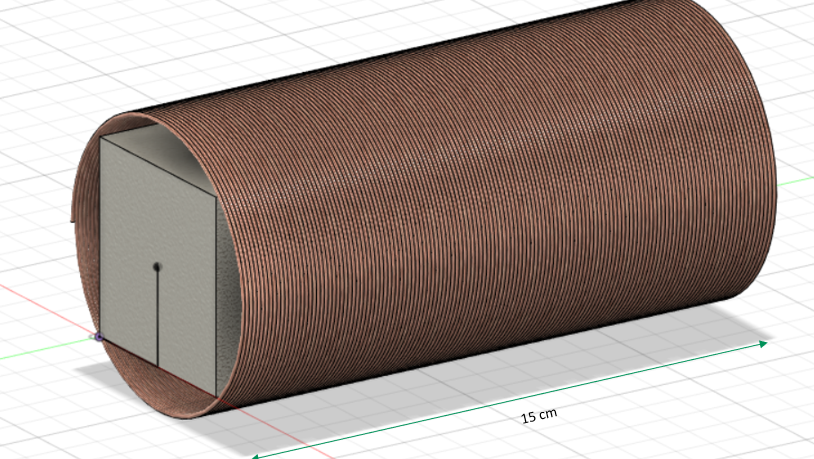
\includegraphics[width=\linewidth]{magnetCAD}
	\caption{CAD of a capturing magnet}
\end{figure}


With those design choices we get the following parameters while taking into consideration that there should not be any kind of residuals in the core alloy :

\begin{itemize}
	\item $\mu_0 = 4\pi \times 10^{-7}\ H/m$
	\item $\mu = \bigg(\frac{\mu_{iron}+\mu_{cobalt}}{2}\bigg)\times\mu_0=5.868\times10^{-3}\ H/m$
	\item $N=135$ turns
	\item $I = 10\ A$
	\item $A = 25cm^2=2.5\times10^{-3}\ m^2$
	\item $\rho_{core} = \rho_{iron}\times 0.9 + \rho_{cobalt}\times0.1 = 7.9726\ g/cm^3$
	\item $\rho_{coil} = \rho_{copper} = 8.96\ g/cm^3$
\end{itemize}

We then need to find the length $L$ of the mean magnetic circuit. In order to do so, we decided to start the capturing sequence at $10\ m$ from the satellite and that the target has an exploitable nozzle of $40\ cm$ of diameters which is realistic for spacecrafts in the mass range of $3\ 500\ kg$. We could then sketch the capturing sequence as so (not to scale) :

\begin{figure}[H]
	\centering
	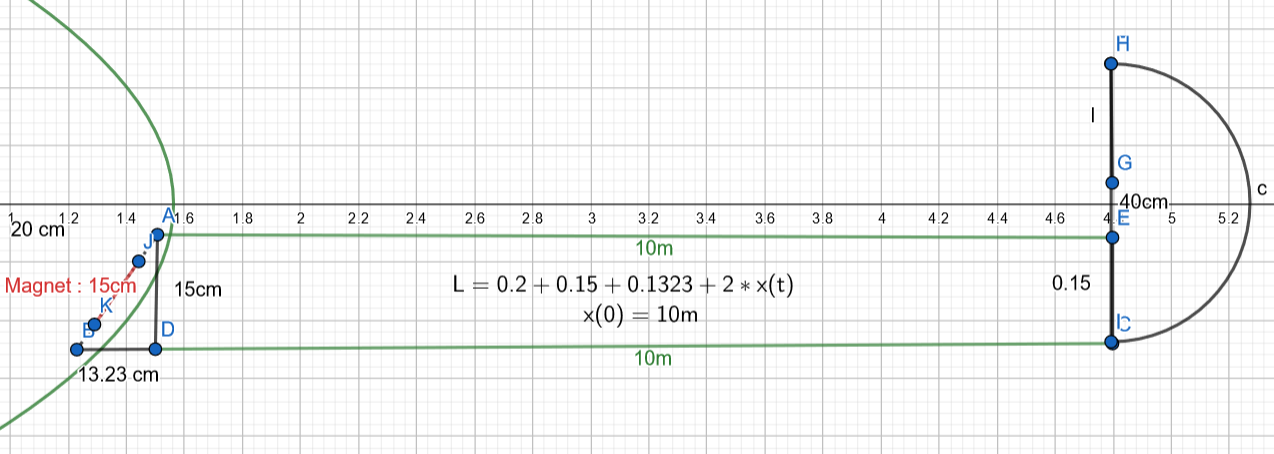
\includegraphics[width=\linewidth]{catching}
	\caption{Capturing sequence (not to scale)}
\end{figure}
We can then have the length $L$ as a function of the distance between the tip of our spacecraft and the nozzle of our target. As a result we can proceed to find the feasibility of our solution with this magnet design by finding the time it would require at this state to attract the target. However, in this case, the current modulation when the target is close has not been modeled due to its complexity.\\

Considering that the force will be on one axis only and $m = 0.001\times m_{target} = 3.5\ kg$ :
\begin{align}
\vec F &= m\vec a\\
\frac{(\mu NI)^2 A}{2\mu_0 L(x)^2} &= m \times \ddot x\\
\frac{(\mu NI)^2 A}{2\mu_0 [0.2 + 0.15 + 0.1323 + 2x(t)]^2} &= m \ddot x(t)\\
\frac{(\mu NI)^2 A}{2\mu_0 [0.4823 + 2x(t)]^2} &= m \ddot x(t)
\end{align}

The capturing time can then be found using $ode45$ on Matlab :
\begin{minted}[fontsize=\footnotesize, linenos, autogobble, breaklines]{matlab}
clearvars; clc;
catchtime = 1;
x0 = 10;
while 1
    [t,x] = ode45(@f3,[0:1:catchtime], [x0; 0; 0; 0]);
        if (x(catchtime ,1) >= 2 * x0)
            break
        else
            catchtime = catchtime +1;
        end
end
\end{minted}
And the function used for the $ode$ solver :
\begin{minted}[fontsize=\footnotesize, linenos, autogobble, breaklines]{matlab}
function  [Xdot] = f3(t, X)
mu = 5.686e-3; mu0 = 4 * pi * 10 ^(-7);
N = 135; I = 10; A = 0.05 ^ 2; m = 3500 ;
x = X(1); y = X(2); vx = X(3); vy = X(4);
Fmag = (mu * N * I) ^2 * A / (2 * mu0 *(2 * norm(X(1:2)) + 0.4823) ^ 2 );
Xdot = [vx; vy;  0.001 * Fmag / m; 0]; 
end
\end{minted}
We then get a capture time of $812$ seconds. As a result, we can determine the energy required to operate the magnets aswell as their masses and volumes. We are considering a holding time for approximately half an hour and we also need to verify that the magnets will be able to hold the target while we are de-orbiting.